En las últimas dos secciones vimos las formalizaciones relacionadas con las EPAs y las capacidades de Manticore.
A continuación, presentaremos dos algoritmos para la construcción de EPAs.
El algoritmo clásico es presentado, con algunas diferencias de notación, como fue presentado por De Caso et. al en 2013 \cite{de-caso-epa}.
El algoritmo novedoso hace uso específicamente de ejecución simbólica y, al haber sido diseñado para Manticore, se adapta a las peculiaridades mencionadas en la sección anterior.

\section{Construcción clásica de EPAs}
\label{sec:algoritmo-clasico}
Tradicionalmente, existe un algoritmo genérico para la construcción de \textit{EPAs} de artefactos de código.
Por cuestiones de notación, para ver el algoritmo de generación de EPAs es conveniente definir el siguiente predicado presentado por De Caso et. al \cite{de-caso-epa} sobre las configuraciones dado un conjunto de precondiciones de un contrato:

\begin{definition}[Predicado de un conjunto de métodos]
    Dados un contrato $SC = \langle M, F, R, inv, init \rangle$ y un conjunto de metodos, $\mathcal{M} \subseteq M$, definimos $pred_\mathcal{M} : \mathcal{C} \rightarrow \{\textbf{true}, \textbf{false}\}$ como
    \[pred_\mathcal{M}(c) \iff inv(c) \land \bigwedge\limits_{m \in \mathcal{M}} \exists p \in \mathds{Z} . R_m(c,p) \land \bigwedge\limits_{   m \notin \mathcal{M}} \nexists p \in \mathds{Z} . R_m(c,p)\]
\end{definition}
El algoritmo, que presentamos a continuación, genera la porción de la EPA que es alcanzable desde $P_0$ (los estados iniciales), realizando \textit{Breadth-First-Search} en el grafo de las transiciones \cite{de-caso-epa}.

\begin{algorithm}[H]
    \caption{Construcción de EPAs}
    \hspace*{\algorithmicindent} \textbf{Input} $SC = \langle M, F, R, inv, init \rangle$ contrato \\
    \hspace*{\algorithmicindent} \textbf{Output} La \textit{EPA} $L_A =\langle \Sigma, S, P_0, \Delta \rangle$
    \begin{algorithmic}[1]
        \State $\Sigma = M$; $S = \emptyset$
        \State $\Delta(s,m) = \emptyset \quad \forall s \in 2^R, m \in M$
        \State $\mathcal{M}^- = \{m \in M | \forall c \: . \: init(c) \Rightarrow \nexists p \in \mathds{Z} \: . \: R_m(c,p)\}$
        \State $\mathcal{M}^+ = \{m \in M | \forall c \: . \: init(c) \Rightarrow \exists p \in \mathds{Z} \: . \: R_m(c,p)\}$
        \State $P_0^c = \{\mathcal{M} \in \#M | \mathcal{M}^+ \subseteq \mathcal{M} \land \mathcal{M}^- \cap \mathcal{M} = \emptyset \}$
        \State $P_0 = \{\mathcal{M} \in P_0^c | \exists c . init(c) \land pred_\mathcal{M}(c) \}$
        \State $W =$ Cola con los elementos de $P_0$
        \While{hay un conjunto $\mathcal{M}$ en la cabeza de $W$}
        \State $S = S \cup \{\mathcal{M}\}$
        \For{$m \in \mathcal{M}$}
        \State $\mathcal{N}^- = \{n \in M | \forall c \in \mathcal{C}, p \in \mathds{Z} \: . \: pred_\mathcal{M}(c) \land R_m(c,p) \Rightarrow \nexists p^\prime \in \mathds{Z} \: . \: R_n(F_m(c,p),p^\prime)\}$
        \State $\mathcal{N}^+ = \{n \in M | \forall c \in \mathcal{C}, p \in \mathds{Z} \: . \: pred_\mathcal{M}(c) \land R_m(c,p) \Rightarrow \exists p^\prime \in \mathds{Z} \: . \: R_n(F_m(c,p),p^\prime)\}$
        \State $S^C = \{\mathcal{N} \in \#M | \mathcal{N}^+ \subseteq \mathcal{N} \land \mathcal{N}^- \cap \mathcal{N} = \emptyset\}$
        \For{$\mathcal{N} \in S^C$}
        \If{$ \exists c \in \mathcal{C} \: . \: pred_\mathcal{M} (c) \land \exists p \in \mathds{Z} \: . \: R_m(c,p) \land pred_\mathcal{N}(F_m(c,p)) $}
            \State $\Delta (\mathcal{M},m) = \Delta (\mathcal{M},m) \cup \mathcal{N}$
            \If{$\mathcal{N} \notin S \land \mathcal{N} \notin W$}
            \State $W.push(\mathcal{N})$
            \EndIf
            \EndIf
            \EndFor
            \EndFor
            \EndWhile
            \State \Return $\langle \Sigma, S, P_0, \Delta \rangle$
    \end{algorithmic}
\end{algorithm}

Aquí, calcular los conjuntos $\mathcal{M}^-$, $\mathcal{M}^+$, $\mathcal{N}^-$ y $\mathcal{N}^+$ es una optimización que permite reducir la cantidad de transiciones candidatas de la EPA \cite{de-caso-epa}.

Decidir si una transición pertenece o no la EPA, como está planteado en el algoritmo, es resolver problemas de validez de fórmulas de primer orden.
Esto en general es indecidible, sin embargo la sugerencia principal consiste en transformar estas preguntas de validez de fórmulas de primer orden en problemas de alcanzabilidad de código, dado que se espera que las precondiciones y los invariantes definidos en la formalización~\ref{definicion-smart-contract} estén debidamente implementados en el contrato.

En general, por optimizaciones de gas, es común que en los métodos externos los contratos definan las precondiciones explícitamente mediante instrucciones \textcolor{magenta}{\texttt{require}}, como en el contrato ejemplo \ref{fig:solidity-example} \texttt{SimpleMarketplace}.
Dado que los inputs externos nunca garantizan estar bien formados, resulta menos costoso para el contrato abortar estas ejecuciones lo antes posible en lugar de hacerlas avanzar hasta llegar a un estado de error.
Sin embargo, debido a que no se espera que sea posible generar instancias que no satisfagan el invariante, por el mismo motivo de ahorro de gas, no es usual contar con una implementación explícita del invariante en el código fuente del contrato.
Tenerlo implicaría ejecutar código que se espera que dé siempre el mismo resultado, por lo que resulta más eficiente no hacerlo.

\section{Algoritmo alternativo}
\label{sec:algoritmo-aternativo}
Implementar el invariante del contrato, además de no ser una práctica estándar, es a menudo exigente para el programador, y es también una actividad propensa a errores.
Sin embargo, es importante en la definición~\ref{definicion-lts} de la semántica de un contrato inteligente la  presencia del invariante.
Intentar construir EPAs incluyendo estados que no satisfagan el invariante suele producir abstracciones demasiado sobreaproximadas \cite{de-caso-epa}.
Por eso, en continuación del trabajo presentado por Godoy et al. \cite{predicate-abstraction-for-smart-contract-validation}, trabajaremos construyendo las EPAs a partir de las precondiciones explícitas dadas por las declaraciones \textcolor{magenta}{\texttt{require}} al comienzo de los métodos, y haciendo uso  del invariante implícito dado por los métodos mismos del contrato.

Trabajemos con la acepción de que un contrato es correcto si la ejecución de todos sus métodos preservan el invariante si se satisfacen las precondiciones del método.
La idea es que bajo la asunción de que un contrato es correcto, ejecutar cualquier sucesión de métodos del contrato con parámetros válidos (es decir, que satisfagan las precondiciones) genera instancias que satisfacen el invariante.
Esto significa que explorar cadenas de transacciones que comienzen por el constructor siempre considera estados que satisfacen el invariante, siempre y cuando cada llamado individual a métodos cumpla las precondiciones correspondientes.
Entonces, es posible asumir que se satisface el invariante si se presenta una traza de llamados válidos a métodos que comienza por el constructor.

Por otro lado, si todos los métodos de un contrato implementan explícitamente sus precondiciones, podemos decir aún mas.
Si este es el caso entonces es imposible que ningún llamado a un método genere un estado inválido.
En su lugar, un llamado que no satisfaga las precondiciones del método será revertido.
De esta manera, \textit{cualquier} traza de métodos que comienze por el constructor genera una instancia del contrato que satisface el invariante, si los métodos implementan explícitamente sus precondiciones.

En esta sección presentamos el algoritmo que construye EPAs haciendo uso de una herramienta de ejecución simbólica, siguiendo la idea esbozada anteriormente para mantener el análisis en estados que satisfagan el invariante.
Dado que trabajaremos asumiendo que no hay acceso explícito al invariante, la nueva formalización que utilizaremos para los contratos inteligentes es la siguiente:

\begin{definition}(Formalización laxa de un contrato inteligente)
    \label{definicion-laxa-smart-contract}
    Definimos a la versión laxa de un contrato inteligente como la tupla $SC = \langle M, F, R, Constructor \rangle$ donde:
    \begin{itemize}
        \item $M, F$ y $R$ son iguales a la definición original
        \item $inv$ no forma parte de $SC$ porque asumimos que se preserva luego de cada llamado a $F_m(c,p)$ independientemente de si $R_m(c,p) = \textbf{true}$
        \item $Constructor \in M$ reemplaza el predicado $init$ y representa un método del contrato que genera las instancias iniciales.
    \end{itemize}
\end{definition}
El LTS concreto (la semántica) y el LTS abstracto (la EPA) de smart contracts que usan esta definición pueden formalizarse de manera análoga a las secciones anteriores.
Por cuestiones de notación, introduciremos algunas funciones sobre los caminos posibles en los métodos de un contrato:
\begin{definition}[Conjunto de posibles caminos de ejecución de una secuencia de funciones]
    Dados un contrato $SC = \langle M, F, R, Constructor \rangle$ definimos la función \texttt{paths\_of} que opera en el dominio de las secuencias de funciones $f_1, f_2, \cdots f_k$ tales que $\forall i, f_i \in F \cup R$:
    \begin{multline}
        \texttt{paths\_of}(f_1, f_2, \cdots f_k) = \{p \: | \: p \text{ es una secuencia de instrucciones del código fuente de SC} \\
        \text{que podría ser un camino que toma la ejecución de } f_1, f_2, \cdots f_k \}
    \end{multline}
\end{definition}
En particular, \texttt{paths\_of} se refiere al conjunto de caminos que son efectivamente factibles.
Es decir, no se consideran caminos de ejecución para los que no exista una serie de inputs que obligan a recorrerlos.
\begin{definition}[Resultado simbólico del camino de ejecución en una secuencia de funciones]
    Dados un contrato $SC = \langle M, F, R, Constructor \rangle$ definimos la función \texttt{sym\_res\_of} que opera en el dominio de los caminos de secuencias de funciones:
    \begin{multline}
        \texttt{sym\_res\_of}(p) = \text{le asocia un valor simbólico a cada función que fue llamada en }p
    \end{multline}
\end{definition}

A continuación usaremos la notación ``$\mathcal{M}=sy$'' donde $\mathcal{M}$ es un estado abstracto de la EPA y $sy$ uno de los estados simbólicos mencionados anteriormente.
Esta notación la usaremos para referirnos a la ``fórmula de compatibilidad'' entre estos dos.
Brevemente, recordemos que un estado de la EPA $\mathcal{M}$ es un subconjunto de los métodos del contrato, y representa los estados concretos en los que los métodos contenidos en el subconjunto se encuentran habilitados, y los demás se encuentran deshabilitados.
Podremos decir que para un camino de ejecución $p$ de las funciones $R_{m\_1},R_{m\_2} \cdots R_{m\_n}$ el resultado simbólico de $p$, $sy = \texttt{symb\_res\_of}(p)$ es compatible con $\mathcal{M}$ sí y sólo sí para cada $R_m$, el resultado de $R_{m\_i}$ en $sy$ es \textbf{true} $\iff m\_i \in \mathcal{M}$.

Consideremos el siguiente ejemplo para el contrato \texttt{Simple\allowbreak Marketplace}:
Sean $\mathcal{M} = \{MakeOffer, Reject\}$ y $p_1$ que representa un camino hasta cierto punto de \texttt{SimpleMarketplace}.
Sea $p_2 \in \texttt{paths\_of}(R_{MakeOffer}; R_{AcceptOffer}; R_{Reject})$ que representa un camino posible de ejecutar las precondiciones del contrato.
Además, sea $sy = \texttt{symb\_res\_of}(p_1;p_2)$, donde con ``$;$'' notamos la concatenación de caminos, tal que los resultados de las precondiciones en $sy$ son $\{R_{MakeOffer} = r_1$, $R_{AcceptOffer} = r_2$, $R_{Reject} = r_3\}$.
La fórmula de compatibilidad entre $\mathcal{M}$ y $sy$ será $\Phi = (r_1 = \textbf{true} \land r_2 = \textbf{false} \land r_3 = \textbf{true} \land sy)$ y significa que en la ejecución de $(R_{MakeOffer}; R_{AcceptOffer}; R_{Reject})$ existen valores de entrada que recorren $p_1;p_2$ y que los resultados dan \textbf{true} para \textcolor{orange}{\texttt{MakeOffer}} y \textcolor{orange}{\texttt{Reject}} y false para \textcolor{orange}{\texttt{AcceptOffer}}.
Dicho de otra manera, esto es que existen parámetros de entrada que generan un estado que se abstrae a $\mathcal{M}$ luego de la ejecución de $p_1$.
Luego, esto quiere decir que si la fórmula $\Phi$ es satisfacible, entonces tenemos garantía de que luego de ejecutar $p_1$ el contrato \textit{puede} encontrarse en un estado que se abstrae a $\mathcal{M}$.
Por otro lado la no satisfacibildad de $\Phi$ indicaría que es imposible llegar al estado de la epa $\mathcal{M}$ luego de ejecutar $p1$.
El algoritmo para expresar la fórmula de compatibilidad entre $p_1$ y $sy$ es el siguiente:

\begin{algorithm}[H]
    \captionsetup{belowskip=0pt}
    \caption{Operador ``$=$'' entre estados de una EPA y resultados simbólicos (ecuación de compatibilidad)}
    \hspace*{\algorithmicindent} \textbf{Input} $SC = \langle M, F, R, Constructor \rangle$ contrato \\
    \hspace*{\algorithmicindent} \textbf{Input} $\mathcal{M}$ un estado de la EPA de $SC$ \\
    \hspace*{\algorithmicindent} \textbf{Input} $sy$ resultado simbolico de una ejecución de $SC$ \\
    \hspace*{\algorithmicindent} \textbf{Output} La fórmula de compatibilidad $\Phi$
    \begin{algorithmic}[1]
        \State $\Phi = sy$
        \For{$m \in M$}
        \State $res_m =$ valor de retorno de la última aparición de $R_m$ en $sy$
        \If{$m \in \mathcal{M}$}
        \State $\Phi = \Phi \land (res_m == \textbf{true})$
        \Else
        \State $\Phi = \Phi \land (res_m == \textbf{false})$
        \EndIf
        \EndFor
        \State \Return $\Phi$
    \end{algorithmic}
\end{algorithm}

Utilizando estas notaciones, podemos presentar el algoritmo\ref{alg:alternativo} que explora la porción de la EPA que es alcanzable desde $P_0$, sin acceso al invariante y haciendo uso de ejecución simbólica.
Este algoritmo realiza una versión	modificada de \textit{Depth-First-Search} en el grafo de las transiciones, explorando varias aristas del grafo a la vez.
En particular, en cada iteración del ciclo principal este algoritmo agrega múltiples transiciones a la EPA etiquetadas por un mismo método.
La exploración siempre se realiza a partir del conjunto de estados de la EPA ``$S_{current}$'' que en cada iteración se actualiza con el conjunto de estados en los que puede resultar la ejecución del último método.
Cuando esta exploración llega a un punto muerto, se retrocede usando la pila del \textit{DFS} hasta otro punto en el que queden llamados de métodos sin explorar.
\begin{algorithm}[H]
\captionsetup{belowskip=0pt}
\caption{Construcción de EPAs mediante ejecución simbólica}
 \hspace*{\algorithmicindent} \textbf{Input} $C = \langle M, F, R \rangle$ contrato \\
 \hspace*{\algorithmicindent} \textbf{Output} La \textit{EPA} $L_A =\langle \Sigma, S, P_0, \Delta \rangle$
 \begin{algorithmic}[1]
\State $\Sigma = M$
\State $S = \emptyset$ $;P_0 = \emptyset$
\State $\Delta(s,m) = \emptyset \quad \forall s \in 2^R, m \in M$
\State $Paths_{pre} = \{p | p$ es un posible camino de ejecución de $F_{Constructor};R\_1;R\_2; \dots R\_n\}$
\State $Symb_{pre} = \{$resultado simbólico luego de ejecutar $p | p \in Paths_{pre} \}$ 
\State $P_0 = \{s \in 2^R | \exists sy \in Symb_{pre} \: . \: SAT(sy= s)\}$
\State $S_{current } = P_0$
\State $marcados = \emptyset$
\State $W =$ Pila vacía ;$W.$Push$((S_{current},Symb_{pre}))$
\While{$W . $NotEmpty$()$}
    \State $S =$ Update con $S_{current }$
    \If{$\exists m \in M\: . \: \{s \in S_{current } | m \in s \land (s,m) \notin marcados\} \neq \emptyset$} 
        \State Elegir tal $m$
        \State $Paths_{post\_m} = \{p | p$ es un posible camino de ejecución de $F_m;R\_1;R\_2; \dots R\_n\}$
        \State $Symb_{post} = \{$resultado simbólico luego de ejecutar $p1;p2 \:|\: p1 \in Paths_{pre} \land p2 \in Paths_{post\_m} \} $
        \State $S_{next} = \emptyset$
        \For{$\{s_1 \in S_{current } | m \in s_1 \land (s_1,m) \notin marcados\}$}
            \State $marcados \pluseq \{(s_1,m)\}$
            \State  $\Delta(s_1,m) = \{s_2 \in 2^R | \exists sy_1 \in Symb_{pre}, sy_2 \in Symb_{post\_m} \: . \: SAT(sy_1= s_1 \land sy_2 = s_2)\}$ 
            \State $S_{next} = \Delta(s_1,m)$
        \EndFor
        \State $S_{current } = S_{next}$
        \State $Symb_{pre} = Symb_{post}$
        \State $Paths_{pre} = (Paths_{Pre};$ $Paths_{Post})$ 
        \State $W.$Push$((S_{current },Symb_{pre}))$
    \Else
        \State $(S_{current },Symb_{pre}) = W.$Pop$()$
    \EndIf
\EndWhile
\State \Return $\langle \Sigma, S, P_0, \Delta \rangle$
\end{algorithmic}
\end{algorithm}
%\begin{tcolorbox}[blanker,
%        float=htb!,
%        grow to left by=1.5cm,
%        grow to right by=1.2cm,
%        top=-1.2cm,
%        bottom=-0.8cm]
%    \begin{algorithm}[H]
\captionsetup{belowskip=0pt}
\caption{Construcción de EPAs mediante ejecución simbólica}
 \hspace*{\algorithmicindent} \textbf{Input} $C = \langle M, F, R \rangle$ contrato \\
 \hspace*{\algorithmicindent} \textbf{Output} La \textit{EPA} $L_A =\langle \Sigma, S, P_0, \Delta \rangle$
 \begin{algorithmic}[1]
\State $\Sigma = M$
\State $S = \emptyset$ $;P_0 = \emptyset$
\State $\Delta(s,m) = \emptyset \quad \forall s \in 2^R, m \in M$
\State $Paths_{pre} = \{p | p$ es un posible camino de ejecución de $F_{Constructor};R\_1;R\_2; \dots R\_n\}$
\State $Symb_{pre} = \{$resultado simbólico luego de ejecutar $p | p \in Paths_{pre} \}$ 
\State $P_0 = \{s \in 2^R | \exists sy \in Symb_{pre} \: . \: SAT(sy= s)\}$
\State $S_{current } = P_0$
\State $marcados = \emptyset$
\State $W =$ Pila vacía ;$W.$Push$((S_{current},Symb_{pre}))$
\While{$W . $NotEmpty$()$}
    \State $S =$ Update con $S_{current }$
    \If{$\exists m \in M\: . \: \{s \in S_{current } | m \in s \land (s,m) \notin marcados\} \neq \emptyset$} 
        \State Elegir tal $m$
        \State $Paths_{post\_m} = \{p | p$ es un posible camino de ejecución de $F_m;R\_1;R\_2; \dots R\_n\}$
        \State $Symb_{post} = \{$resultado simbólico luego de ejecutar $p1;p2 \:|\: p1 \in Paths_{pre} \land p2 \in Paths_{post\_m} \} $
        \State $S_{next} = \emptyset$
        \For{$\{s_1 \in S_{current } | m \in s_1 \land (s_1,m) \notin marcados\}$}
            \State $marcados \pluseq \{(s_1,m)\}$
            \State  $\Delta(s_1,m) = \{s_2 \in 2^R | \exists sy_1 \in Symb_{pre}, sy_2 \in Symb_{post\_m} \: . \: SAT(sy_1= s_1 \land sy_2 = s_2)\}$ 
            \State $S_{next} = \Delta(s_1,m)$
        \EndFor
        \State $S_{current } = S_{next}$
        \State $Symb_{pre} = Symb_{post}$
        \State $Paths_{pre} = (Paths_{Pre};$ $Paths_{Post})$ 
        \State $W.$Push$((S_{current },Symb_{pre}))$
    \Else
        \State $(S_{current },Symb_{pre}) = W.$Pop$()$
    \EndIf
\EndWhile
\State \Return $\langle \Sigma, S, P_0, \Delta \rangle$
\end{algorithmic}
\end{algorithm}
%\end{tcolorbox}

La decisión de explorar los estados de la EPA de esta manera conjunta se debe a las capacidades de la API programable de Manticore.
Al ejecutar un método, debemos ejecutarlo en todos los caminos hasta el momento.
Por este motivo es que exploramos las transiciones desde todos los estados del conjunto ``$S_{current}$'' cada vez, en lugar de realizar una exploración más tradicional en el grafo de transiciones.

Por último, podemos señalar que para garantizar \textit{soundness} de las EPAs generadas, lo tradicional es consultar por la insatisfacibilidad de que una transición pertenezca a la EPA, e incluirla en el resultado en cualquier caso en el que no se pueda demostrar esto.
Sin embargo, en este caso sólo estamos incluyendo las transiciones para las que tengamos una demostración de su existencia.
Esta decisión, aunque discutible, fue prinicipalmente tomada para aprovechar la funcionalidad de generación de casos de test concretos de Manticore.

%El estado inicial y la función de transición comienzan vacíos.
%El conjunto ${Paths_{pre}}$ contiene todos los caminos posibles que puede tomar la ejecución del constructor seguida por la ejecución de las precondiciones de los métodos.
%Si llamamos $init$ al estado (simbólico) luego de ejecutar $F_{Constructor}$, en $Symb_{pre}$ hay para cada uno de los caminos en $Path_{pre}$ una expresión que representa el resultado de la ejecución realizada. Esa expresión es de la forma $(R_1(init) = r_1 , R_2(init) = r_2 \cdots , R_n(init) = r_n)$ .
%Luego, puede calcularse $P_0$ mediante una sucesión de preguntas de satisfacibilidad de fórmulas.
%En particular, para cada expresión $sy \in Symb_{pre}$, nos interesa saber con qué estado de la EPA es consistente $sy$.

%Habiendo determinado $P_0$, el algoritmo marca $S_{current}$ como el conjunto de estados de la EPA con los que se corresponde $Symb_{pre}$, y agrega ambos a la pila $W$, que representa conjuntos de estados de la EPA por visitar.
%Para continuar la exploración desde $S_{current}$, se elige uno de los métodos que esté habilitado en alguno de los estados de $S_{current}$ y no se haya explorado ya.
%Luego, para cada estado $s \in S_{current}$ que permite la ejecución de $m$, se calculan los nuevos estados a los que se puede llegar ejecutando $m$, de manera similar a la que se calcula $P_0$.

%El conjunto $Symb_{post}$ de la línea 15 representa los resultados de continuar la ejecución donde la había dejado $Symb_{pre}$.
%En la línea 19, donde se calculan las próximas transiciones, es necesario revisar no sólo la satisfacibildad de que el estado simbólico nuevo sea compatible con el estado de la EPA objetivo, sino que es necesario que aún se mantenga la compatibilidad entre el estado simbólico viejo y el estado de la EPA desde el que se está transisionando.
%Esto es porque las expresiones en $Symb_{pre}$ pueden ser compatibles con $s_1$, pero puede ocurrir una contradicción al pedir que $Symb_{post}$ sea compatible con $s_2$ también.
%De no exigir esto, consideraríamos que valores de entrada que permiten alcanzar $s_2$ pero que nunca alcanzaban $s_1$ previamente indican una transición entre $s_1$ y $s_2$.

\section{Limitaciones}
\label{sec:subaproximacion}
La mayor evidente diferencia entre el algoritmo presentado en la seccion \ref{sec:algoritmo-aternativo} y el algoritmo clásico es que en lugar de poder explorar transiciones entre estados completamente abstractos, la manera en la que explora las transiciones de la EPA implica que sólo está considerando ciertos caminos de métodos al evaluar cada transición.
Esto se debe a que en cada paso selecciona un par (método, estado abstracto) que no haya explorado ya, pero la exploración considera todos los estados posibles que puedan abstraerse al estado abstracto.
En cambio, sólo puede considerarse un subconjunto de los estados que la herramienta pudo alcanzar hasta ese momento.

Consideremos el siguiente ejemplo, el contrato \texttt{BoundedStack}, cuyo código podemos ver en el fragmento de código \ref{code:solidity-bounded-stack}.
Este contrato consiste en una simple implementación de una pila como estructura de datos, con la peculiaridad de que la pila cuenta con un tamaño máximo.
El contrato tiene sólo dos métodos externos: \textcolor{orange}{\texttt{push}} y \textcolor{orange}{\texttt{pop}}.
La EPA de este contrato por otro lado también es bastante sencilla, y la podemos ver en la imagen \ref{fig:bounded-stack-epa}.
Por fuera de los estados \textbf{init} y \textbf{vacio}, contamos con solo tres estados alcanzables, que son \textbf{\_push}, \textbf{\_pop} y \textbf{\_push\_pop}.
El estado \textbf{\_push} se corresponde con la pila vacía, y es el que se produce al desplegar el contrato o luego de ejecutar \textcolor{orange}{\texttt{pop}} reiteradas veces.
Cuando la pila tiene elementos pero no está llena se encuentra en el estado \textbf{\_push\_pop}, al que se puede llegar tanto desde sí mismo, como desde \textbf{\_push} y desde \textbf{\_pop}.
Finalmente, el estado \textbf{\_pop} se corresponde con la pila llena, y se puede llegar tanto desde \textbf{\_push} (si el tamaño de la pila fuese uno) o desde \textbf{\_push\_pop}, pero no desde el constructor.
Notoriamente, a menos que el contrato sea deployeado con un tamaño máximo de cero, nunca será posible alcanzar el estado \textbf{\_vacio}.

\begin{lstlisting}[language=Solidity, label={code:solidity-bounded-stack}, caption={Contrato Inteligente \texttt{BoundedStack} en Solidity},captionpos=b]
contract SizedStack {
    uint256 public size;
    uint256 public maxSize;
    uint256[] internal_arr;
    constructor() public {
        maxSize = 10;
        size = 0;
    }
    function isEmpty() public view returns (bool) {
        return size == 0;
    }
    function top() public view returns (uint256) {
        require(!isEmpty());
        return internal_arr[size - 1];
    }
    function push(uint256 new_elem) public {
        require(size < maxSize);
        internal_arr.push(new_elem);
        size += 1;
    }
    function pop() public returns (uint256) {
        require(!isEmpty());
        uint256 was = top();
        internal_arr.pop();
        size -= 1;
        return was;
    }
}
\end{lstlisting}


Este es un buen ejemplo para observar la limitación introducida por el algoritmo alternativo al no explorar realmente todas las ejecuciones posibles de un método.
Como se representa en la figura \ref{fig:bounded-stack-bad-epa}, veremos que es posible que el análisis del contrato \texttt{BoundedStack} por el algoritmo alternativo no pueda encontrar algunas de las transiciones presentes en la EPA, dependiendo del orden en el que elija ejecutar los métodos del contrato.
Realicemos manualmente la exploración que realizaría el algoritmo para este contrato y veamos que es posible llegar al resultado presentado en la figura \ref{fig:bounded-stack-bad-epa}, en el que algunas transiciones son omitidas de la EPA.

El algoritmo explora los estados alcanzables comenzando desde el constructor.
Como vimos en la EPA de \texttt{BoundedStack}, los estados que resultan alcanzables son \textbf{\_push} y \textbf{vacio}.
Hasta ahora tenemos entonces $P_0 = \{\emptyset, \textbf{\_push}\}, S = \{\emptyset, \textbf{\_push}\}$ y que  $\Delta(s,m) = \emptyset$ para todos los $m$ y $s$.
Luego, el algoritmo elige un método de los disponibles a ejecutar al azar, que en este caso sería solamente \textcolor{orange}{\texttt{push}}.
Luego de ejecutar ese método, los estados que resultan alcanzables desde el estado \textbf{\_push} son \textbf{\_push\_pop} (con la restricción de que el tamaño de la pila sea mayor a uno) y \textbf{\_pop} (con la restricción de que el tamaño de la pila sea exactamente uno).
En este punto, $P_0 = \{\emptyset, \textbf{\_push}\}, S = \{\emptyset, \textbf{\_push}, \textbf{\_push\_pop}, \textbf{\_pop}\}$ y  $\Delta(\textbf{\_push},\textcolor{orange}{\texttt{push}}) = \{\textbf{\_push\_pop}, \textbf{\_pop}\}$.

Ahora, este es el punto en el que el próximo paso de la exploración del algoritmo puede cambiar el resultado final de la abstracción generada.
Por un lado, podemos elegir explorar \textcolor{orange}{\texttt{pop}} desde \textbf{\_push\_pop} y \textbf{\_pop}, marcando los pares $(\textbf{\_push\_pop},\textcolor{orange}{\texttt{pop}})$ y $(\textbf{\_pop},\textcolor{orange}{\texttt{pop}})$ como ya explorados, o explorar \textcolor{orange}{\texttt{push}} desde \textbf{\_push\_pop} y dejar la exploración de \textcolor{orange}{\texttt{push}} para más adelante.
Por otro lado se puede explorar \textcolor{orange}{\texttt{push}}, marcando el par $(\textbf{\_push\_pop},\textcolor{orange}{\texttt{push}})$.
Si continuamos la ejecución suponiendo que en este paso se elige explorar \textcolor{orange}{\texttt{pop}}, descubriremos dos transiciones nuevas: de \textbf{\_push\_pop} a \textbf{\_push} mediante \textcolor{orange}{\texttt{pop}} y de \textbf{\_pop} a \textbf{\_push} mediante \textcolor{orange}{\texttt{pop}} también.
Nos puede llamar la atención que desde los estados (concretos) que elegimos para explorar la ejecución de \textcolor{orange}{\texttt{pop}} hay dos transiciones que no podemos ver: de \textbf{\_pop} a \textbf{\_push\_pop} mediante \textcolor{orange}{\texttt{pop}} y de de \textbf{\_push\_pop} a \textbf{\_push\_pop} mediante \textcolor{orange}{\texttt{pop}}.
Estas se deben a que en este momento todos los estados concretos que estamos considerando tienen su tamaño real de la pila en 1.
Sin embargo, el algoritmo no presta atención a cuál fue la traza de métodos ejecutada para llegar hasta acá, por lo que marca a ambas tuplas $(\textbf{\_push\_pop},\textcolor{orange}{\texttt{pop}})$ y $(\textbf{\_pop},\textcolor{orange}{\texttt{pop}})$ como ya exploradas.
Esto significa que la función de transición $\Delta$ quedará definida en $\Delta(\textbf{\_push\_pop},\textcolor{orange}{\texttt{pop}}) = \textbf{\_push}$ y $\Delta(\textbf{\_pop},\textcolor{orange}{\texttt{pop}}) = \textbf{\_push}$.
De aquí en adelante la ejecución del algoritmo proseguirá hasta terminar con (al menos) esas dos transiciones faltantes.


\begin{figure}
    \centering
    \begin{subfigure}{0.45\textwidth}
        {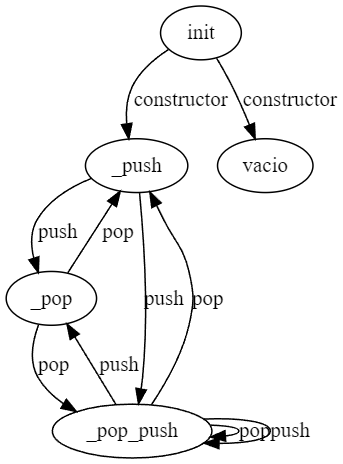
\includegraphics[width=\textwidth]{figs/bounded-stack-good-epa.png}}
        \caption{Enabledness Preserving Abstraction del contrato \texttt{BoundedStack}}
        \label{fig:bounded-stack-epa}
    \end{subfigure}
    \hfill
    \begin{subfigure}{0.45\textwidth}
        {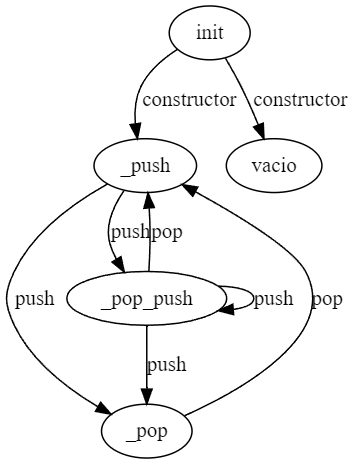
\includegraphics[width=\textwidth]{figs/bonded-stack-bad-epa.png}}
        \caption{EPA errónea del contrato \texttt{BoundedStack} generada por el algoritmo alternativo.
            No se encuentran presentes las transiciones \textbf{\_pop} a \textbf{\_push\_pop} mediante \textcolor{orange}{\texttt{pop}} ni \textbf{\_push\_pop} a \textbf{\_push\_pop} mediante \textcolor{orange}{\texttt{pop}}.}
        \label{fig:bounded-stack-bad-epa}
    \end{subfigure}
\end{figure}
